\documentclass[10pt,journal,compsoc]{IEEEtran}

\ifCLASSOPTIONcompsoc
  \usepackage[nocompress]{cite}
\else
  \usepackage{cite}
\fi

\usepackage[utf8]{inputenc}
\usepackage[T1]{fontenc}
\usepackage{amsmath,amssymb,amsfonts}
\usepackage{algorithm}
\usepackage{algpseudocode}
\usepackage{graphicx}
\usepackage{booktabs}
\usepackage{multirow}
\usepackage{array}
\usepackage{xcolor}
\usepackage[hidelinks]{hyperref}

\graphicspath{{00_manuscript/figures/workflow/}{00_manuscript/figures/pareto_4d_plots/}}

\begin{document}

\title{CAPQ-Pareto: Context-Aware Post-Quantum and Homomorphic Encryption Orchestration for Hybrid Structured-Unstructured Databases Across the Cloud-Edge Continuum}

\author{Preecha~[Surname],~\IEEEmembership{Member,~IEEE}%
\IEEEcompsocitemizethanks{\IEEEcompsocthanksitem P. [Surname] is with Mahasarakham University, Kham Riang, Kantarawichai, Maha Sarakham 44150, Thailand.\protect\\
E-mail: preecha@msu.ac.th}%
\thanks{Target Venue: IEEE Transactions on Cloud Computing (Regular Paper, 12-Page Budget). Artifact Repository: \url{https://github.com/preecha-msu/CAPQ-Pareto}.}}

\markboth{IEEE TRANSACTIONS ON CLOUD COMPUTING (PROPOSAL \& MANUSCRIPT BLUEPRINT)}%
{PREECHA: CAPQ-PARETO ORCHESTRATION FOR HYBRID CLOUD-EDGE DATABASES}

% IEEE Computer Society Strict Rule: 100-200 words, plain text (no citations/equations)
\IEEEtitleabstractindextext{%
\begin{abstract}
Cloud-edge applications such as Retrieval-Augmented Generation (RAG) and clinical analytics increasingly rely on hybrid databases that jointly serve lossless structured transactions (SQL/JSON) and approximate vector similarity queries across wide-area networks (WAN). However, securing these pipelines against quantum adversaries introduces severe cloud-edge bottlenecks: standardized Post-Quantum Cryptography (NIST FIPS 203 ML-KEM) causes handshake expansion and WAN packet fragmentation, whereas zero-trust vector evaluation via approximate Fully Homomorphic Encryption (CKKS) incurs prohibitive latency, edge energy drain, and cloud billing costs while breaking server-side graph indices. We propose CAPQ-Pareto, a context-aware orchestration framework that dynamically routes hybrid database workloads across heterogeneous cryptographic and compression regimes. We formulate joint encryption-quantization selection as a constrained multi-objective Pareto optimization problem minimizing tail latency, physical edge energy, and per-second cloud compute and egress costs under strict security, deadline, and retrieval accuracy (Recall@K) bounds. An online SLA-gated Contextual Bandit scheduler dispatches batches across micro-batched QUIC 0-RTT with hybrid X25519/ML-KEM-768, precision-quantized vector transport over lightweight PQC, and coarse-bucketed CKKS inner-product search. Evaluation spans bare-metal Intel RAPL edge containers and multi-region Google Cloud x86\_64 and ARM64 clusters running PostgreSQL (pgvector) and Milvus.
\end{abstract}

\begin{IEEEkeywords}
Cloud-edge continuum, post-quantum cryptography, ML-KEM, homomorphic encryption, hybrid vector databases, multi-objective optimization, cloud economics, tail latency.
\end{IEEEkeywords}}

\maketitle
\IEEEdisplaynontitleabstractindextext
\IEEEpeerreviewmaketitle

\IEEEraisesectionheading{\section{Introduction and Problem Statement}\label{sec:introduction}}
\IEEEPARstart{C}{loud-edge} data infrastructures supporting enterprise Retrieval-Augmented Generation (RAG) and smart healthcare workflows simultaneously execute structured metadata queries (SQL/JSON requiring $100\%$ lossless integrity) and approximate nearest-neighbor (ANN) vector searches ($128$--$1024$ dimensions) across hybrid engines such as PostgreSQL (\texttt{pgvector}) and Milvus~\cite{wang2021milvus, malkov2020hnsw}. Protecting long-lived cloud-edge traffic against \textit{Harvest-Now, Decrypt-Later} quantum adversaries and honest-but-curious cloud operators necessitates transitioning to NIST ML-KEM~\cite{nist_fips203_2024, stebila2016liboqs} and approximate Homomorphic Encryption (CKKS)~\cite{cheon2017ckks, badawi2022openfhe}.

Nevertheless, static cryptographic deployment introduces three cloud-system challenges: (1) PQC key/ciphertext expansion triggers IP/TCP packet fragmentation over WAN links, inflating p99 tail latency for small SQL transactions; (2) edge vector quantization (\texttt{FP32} to \texttt{INT8}/1-bit), CKKS approximation noise (which precludes server-side HNSW graph traversal), and hard SLA timeouts couple security directly to effective retrieval accuracy; and (3) prior studies neglect joint optimization across retrieval accuracy, tail latency, physical edge energy (mJ), and per-second cloud compute/egress billing (USD).

\subsection{Key Scientific Contributions}
\begin{itemize}
    \item \textbf{Multi-Region Cloud-Edge Bottleneck Characterization:} Empirical analysis of NIST ML-KEM over QUIC~\cite{iyengar2021quic} and OpenFHE CKKS~\cite{badawi2022openfhe} under dynamic hybrid SQL/vector bursts~\cite{cooper2010ycsb, jegou2011sift, chen2024bgem3} across x86\_64 and ARM64 cloud nodes.
    \item \textbf{Constrained 4D Cloud-Edge Cost-Energy Model:} Joint cryptographic-quantization formulation integrating hardware Intel RAPL energy~\cite{khan2018rapl} and per-second Google Cloud billing under security, p95/p99 deadline, and $\text{Recall@}K$ guarantees.
    \item \textbf{SLA-Gated Contextual Bandit Scheduler:} A sub-millisecond LinUCB orchestrator~\cite{li2010linucb} dynamically routing batches across three cryptographic regimes to minimize SLA violations and cloud operational cost.
\end{itemize}

\section{Related Work and Gap Matrix}
Table~\ref{tab:gap_analysis} positions CAPQ-Pareto relative to existing cloud database and post-quantum networking approaches.

\begin{table*}[t]
\centering
\caption{Comparison of Cloud-Edge Encrypted Database Paradigms vs. Proposed CAPQ-Pareto Framework}
\label{tab:gap_analysis}
\begin{tabular}{lcccccc}
\toprule
\textbf{Paradigm / Scope} & \textbf{Hybrid DB} & \textbf{NIST PQC} & \textbf{Zero-Trust FHE} & \textbf{Tail-SLA \& Recall@$K$} & \textbf{Hardware RAPL} & \textbf{Cloud Billing} \\
\midrule
Classical Cloud DB (TLS 1.3) & \checkmark & $\times$ & $\times$ & $\times$ & $\times$ & Partial \\
Static PQC-TLS / QUIC~\cite{stebila2016liboqs, iyengar2021quic} & $\times$ & \checkmark & $\times$ & $\times$ & Partial & $\times$ \\
Standalone FHE Vector Search~\cite{cheon2017ckks, badawi2022openfhe} & $\times$ & \checkmark & \checkmark & Partial & $\times$ & $\times$ \\
\textbf{CAPQ-Pareto (Proposed)} & \textbf{\checkmark} & \textbf{\checkmark} & \textbf{\checkmark} & \textbf{\checkmark} & \textbf{\checkmark} & \textbf{\checkmark} \\
\bottomrule
\end{tabular}
\end{table*}

\section{System Architecture and Cloud-Edge Formulation}
\begin{figure*}[t]
\centering
\IfFileExists{00_manuscript/figures/workflow/capq_pareto_workflow.jpg}{%
    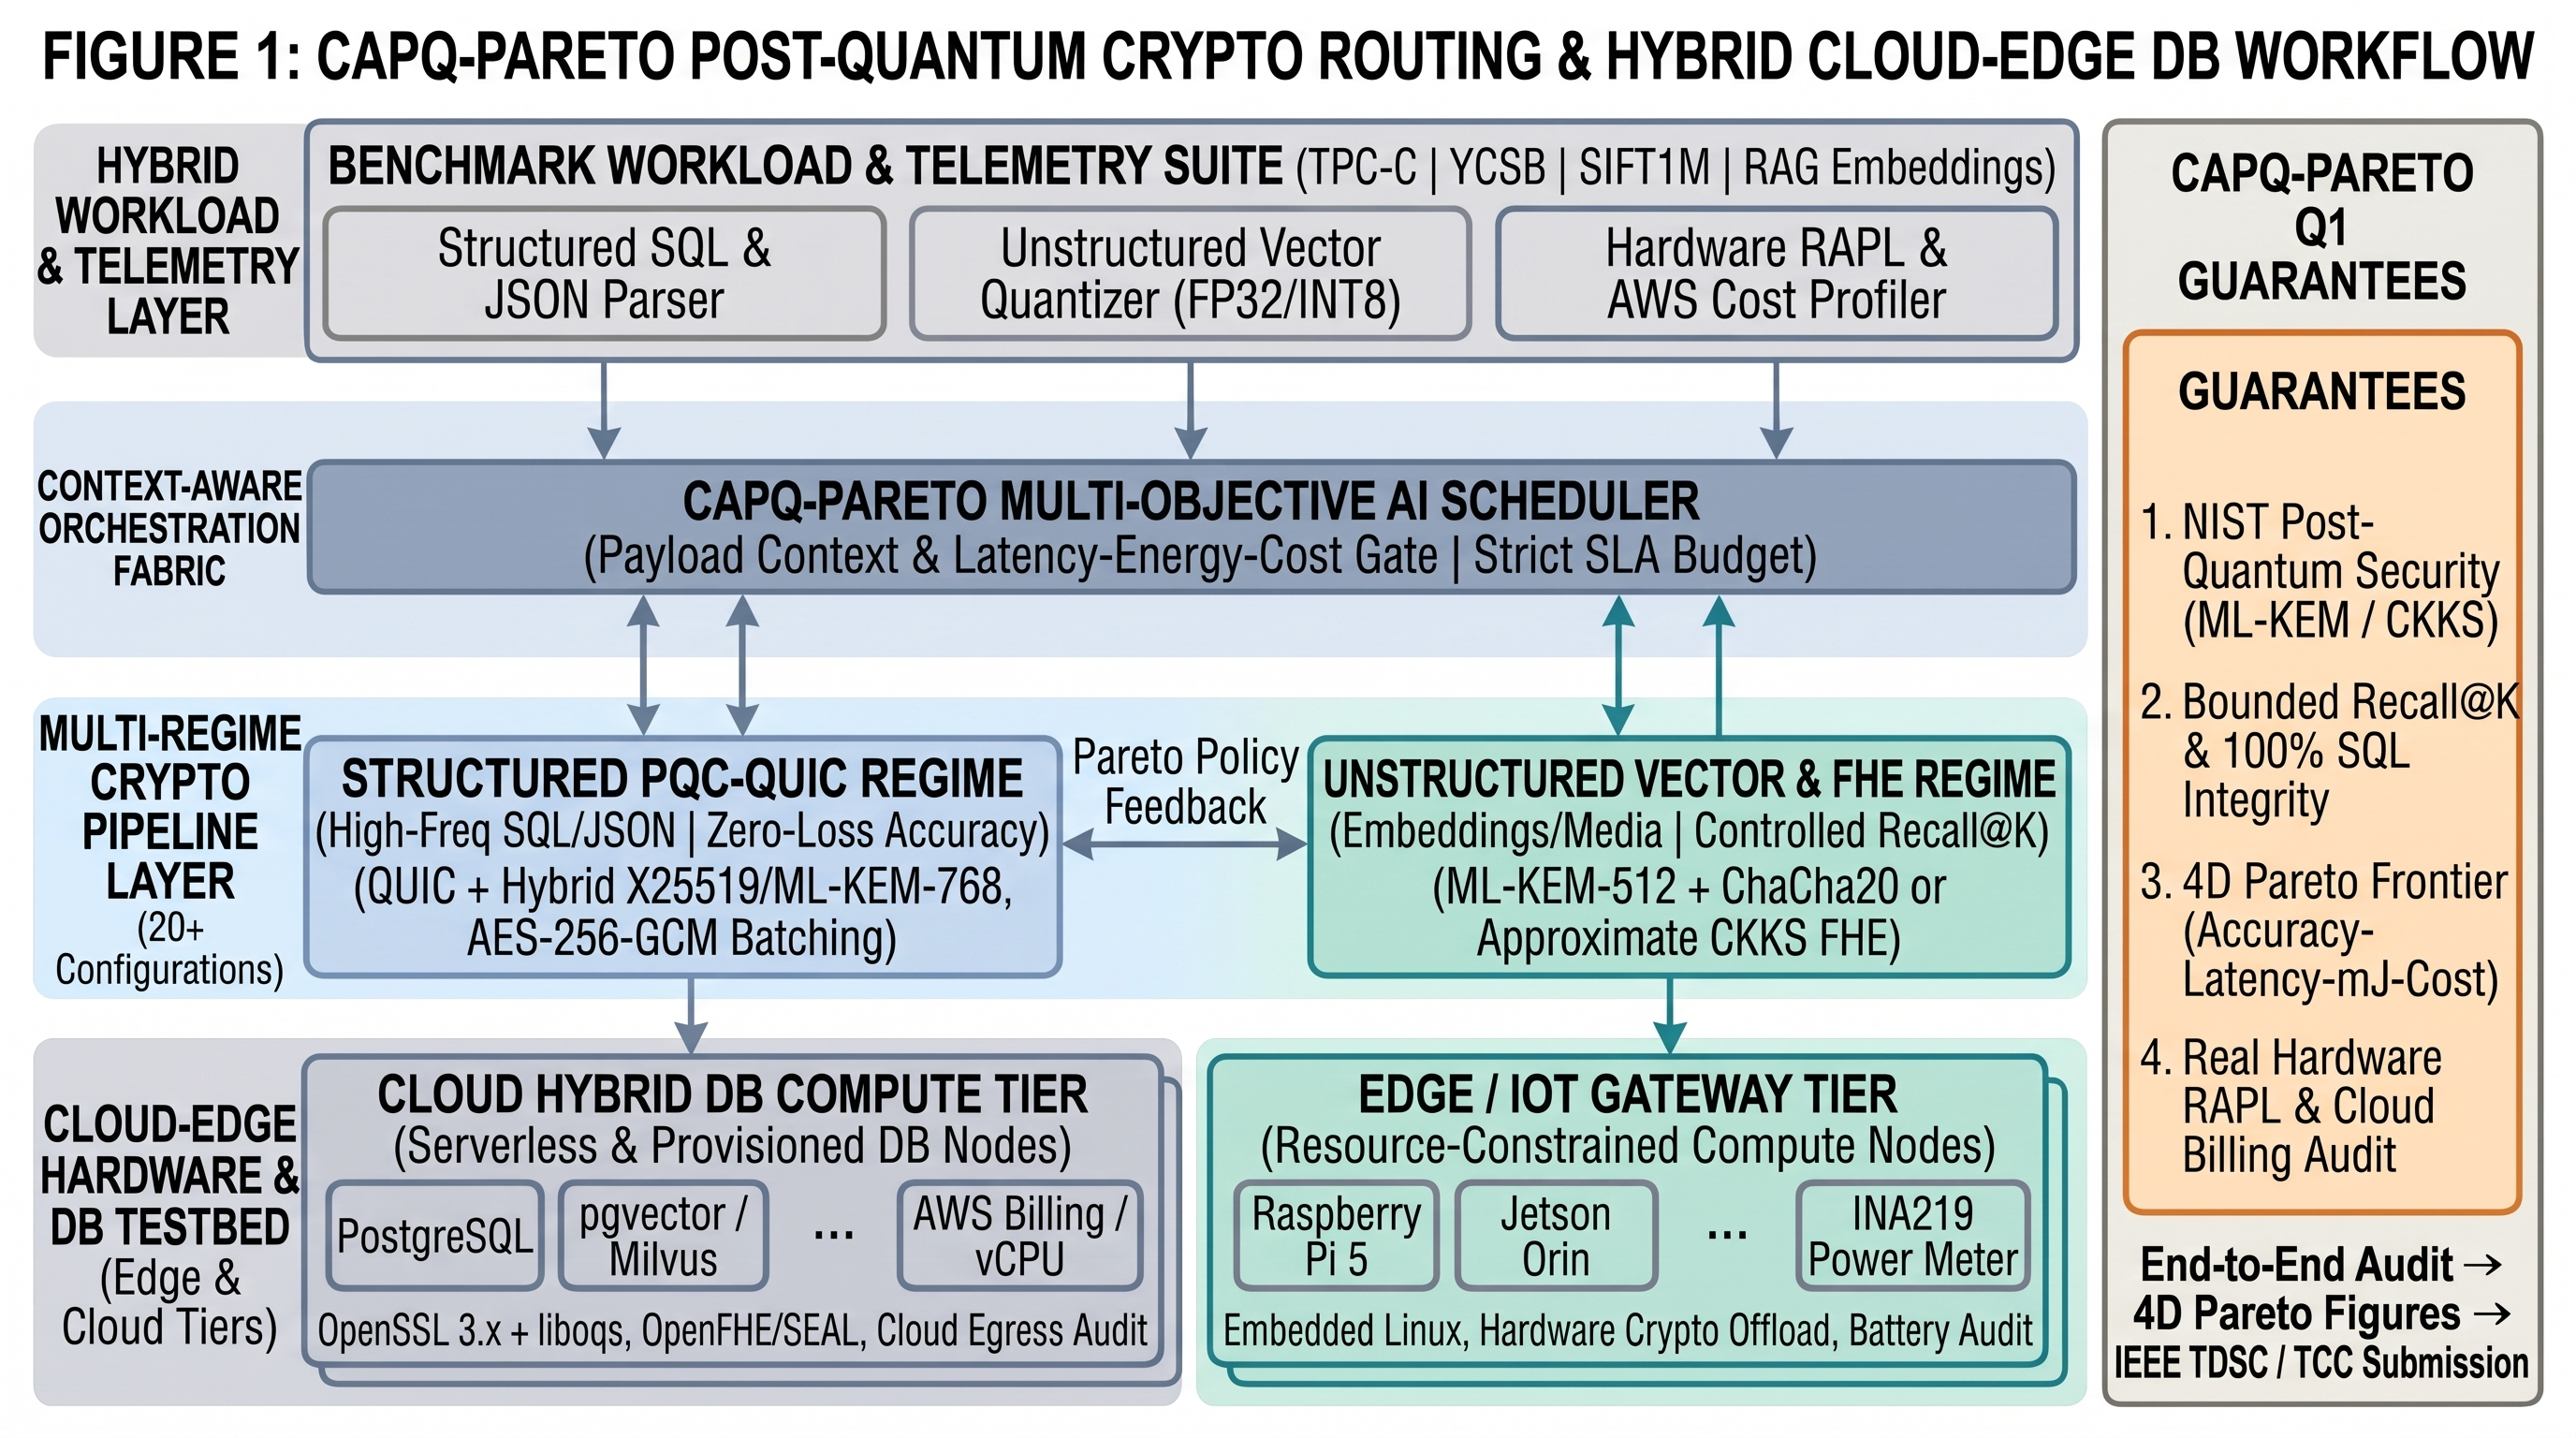
\includegraphics[width=0.95\textwidth]{capq_pareto_workflow.jpg}%
}{%
    \fbox{\parbox{0.94\textwidth}{\centering\vspace{1.0em}
    \textbf{[Figure 1 Placeholder: CAPQ-Pareto 4-Layer Workflow]}\\
    \footnotesize Place \texttt{capq\_pareto\_workflow.jpg} in \texttt{00\_manuscript/figures/workflow/} to render automatically.
    \vspace{1.0em}}}%
}
\caption{CAPQ-Pareto post-quantum cryptographic routing and hybrid Cloud-Edge database workflow.}
\label{fig:architecture}
\end{figure*}

Under instantaneous network state $\boldsymbol{\omega}_t = (\text{BW}_t, \text{RTT}_t, \text{Loss}_t)$ and workload arrival rate $\lambda_t$, CAPQ-Pareto selects regime $m \in \mathcal{M}$ for batch $d_i$ minimizing:
\begin{equation}
\min_{m \in \mathcal{M}} \quad \mathcal{J}(d_i, m \mid \boldsymbol{\omega}_t) = \alpha \hat{L}(d_i, m) + \beta \hat{E}_{\text{edge}}(d_i, m) + \gamma \hat{C}_{\text{gcp}}(d_i, m)
\label{eq:obj}
\end{equation}
subject to $S(m) \ge S_{\text{req}}(d_i)$, $A_{\text{raw}}(d_i, m)\cdot\mathbb{I}[L(d_i,m) \le T_{\max}] \ge A_{\min}(d_i)$, and $L_{\text{p95}}(d_i, m) \le T_{\max}$. Net physical edge energy is measured via RAPL counters $E_{\text{edge}} = \Delta E_{\text{RAPL}} - P_{\text{idle}}\Delta t$, while cloud operational cost models per-second GCP vCPU, memory, and WAN egress charges:
\begin{equation}
C_{\text{gcp}}(d_i, m) = p_{\text{vcpu}} n_{\text{vcpu}} T_{\text{cloud}} + p_{\text{mem}} M_{\text{gb}} T_{\text{cloud}} + p_{\text{egress}} B_{\text{out}}(d_i, m).
\end{equation}

\section{SLA-Gated Orchestrator and Evaluation Plan}
\begin{algorithm}[t]
\caption{CAPQ-Pareto SLA-Gated LinUCB Scheduler}
\label{alg:scheduler}
\begin{algorithmic}[1]
\Require Weights $(\alpha, \beta, \gamma)$, exploration $\nu$, action set $\mathcal{M}$
\For{each incoming hybrid workload batch $d_t$ under burst rate $\lambda_t$}
    \State Observe context $\mathbf{x}_t$ and filter feasible set $\mathcal{M}_{\text{sla}} \subseteq \mathcal{M}$ satisfying security, $A_{\min}$, and $T_{\max}$
    \For{each $m \in \mathcal{M}_{\text{sla}}$}
        \State $\hat{\boldsymbol{\theta}}_m \leftarrow \mathbf{A}_m^{-1}\mathbf{b}_m$; \quad $u_m \leftarrow \hat{\boldsymbol{\theta}}_m^\top \mathbf{x}_t - \nu \sqrt{\mathbf{x}_t^\top \mathbf{A}_m^{-1}\mathbf{x}_t}$
    \EndFor
    \State Dispatch $m^*_t \leftarrow \arg\min_{m \in \mathcal{M}_{\text{sla}}} u_m$ via Regime A (QUIC 0-RTT + ML-KEM-768), Regime B (Quantized ML-KEM-512 + ChaCha20), or Regime C (Bucketed OpenFHE CKKS)
    \State Log $(L_t, E_{\text{edge},t}, C_{\text{gcp},t}, A_{\text{eff},t})$, compute $\mathcal{J}_t$, and update $(\mathbf{A}_{m^*_t}, \mathbf{b}_{m^*_t})$
\EndFor
\end{algorithmic}
\end{algorithm}

\begin{table}[t]
\centering
\caption{IEEE TCC Experimental Matrix (Local RAPL + Multi-Region GCP)}
\label{tab:testbed}
\begin{tabular}{ll}
\toprule
\textbf{Dimension} & \textbf{Specification} \\
\midrule
Local Edge Tier & Bare-metal Linux Docker (\texttt{2 vCPU, 2GB}), Intel RAPL, \texttt{tc/netem} \\
GCP Regions & \texttt{asia-southeast3} (BKK), \texttt{asia-southeast1} (x86/ARM64), \texttt{us-central1} \\
DBs \& Workloads & PostgreSQL (\texttt{pgvector}) \& Milvus; TPC-C, YCSB-A, SIFT1M, BGE-M3 \\
Cloud Metrics & Mean/p95/p99 Latency, SLA Violation \%, RAPL mJ, GCP USD/1M queries \\
Statistical Audit & $720$ core + $450$ ablation runs ($30$ trials/config, Wilcoxon $p < 0.05$) \\
\bottomrule
\end{tabular}
\end{table}

\bibliographystyle{IEEEtran}
\bibliography{references}

\begin{IEEEbiographynophoto}{Preecha [Surname]}
(Member, IEEE) is with Mahasarakham University, Thailand. His research interests include cloud-edge continuum systems, post-quantum security, and distributed database optimization.
\end{IEEEbiographynophoto}

\end{document}